\documentclass[IB,BIB]{TFUOC}%IB: CASTELLANO, CAT: CATALÁN, ENG: ANGLÈS

%Introducción de datos del trabajo
\title{Predicción jerárquica de demanda en retail mediante modelos basados en árboles y redes LSTM con reconciliación jerárquica e interpretabilidad SHAP: aplicación al dataset M5 Forecasting (Walmart)}
\titcrt{Predicción jerárquica de demanda} %Título corto que aparecerá a la cabecera
\author{Tatyana Silchenko Kozyrieva}
\date{1 de marzo de 2026}


\nomPDC{Aarón Montero Montero}
\nomPRA{Susana Acedo}
\titulac{Máster en Ciencia de Datos}
\area{Área 1}

\idioma{Castellano}
\credits{12}
\parcla{time series forecasting; retail demand; machine learning; XGBoost; LightGBM; SHAP values; M5 Forecasting; interpretability; hierarchical forecasting; forecast reconciliation}

\licenc{ccBy}
%Posibles licencias
%ccByNcNd
%ccByNcSa
%ccByNc
%ccByNd
%ccBySa
%ccBy
%GNU
%copyright


%%%%%%%%%%
% Resumen en el idioma

\abstractidioma{
Este Trabajo Final de Máster desarrolla un sistema de predicción jerárquica de demanda en retail utilizando el dataset M5 Forecasting – Walmart, caracterizado por su estructura multinivel y su elevada dimensionalidad temporal y categórica.
El proyecto implementará y evaluará modelos basados en árboles de decisión (Random Forest, XGBoost y LightGBM) para la predicción simultánea de múltiples series temporales, priorizando eficiencia computacional y capacidad de generalización.
De forma complementaria, se implementará un modelo basado en redes neuronales recurrentes (LSTM) con el objetivo de comparar su capacidad para capturar dependencias temporales de largo plazo frente a los modelos tabulares.
Se incorporará reconciliación jerárquica mediante el método MinT (Minimum Trace), utilizando Bottom-Up como referencia comparativa, con el objetivo de garantizar coherencia estructural entre los distintos niveles de agregación del dataset.
Se incorporará un análisis de interpretabilidad mediante SHAP para cuantificar la contribución marginal de las variables explicativas y analizar la estabilidad del modelo en distintos niveles jerárquicos.
El trabajo se orienta a construir una solución reproducible, evaluable mediante métricas estándar del dominio (RMSE, MAE y WRMSSE, métrica oficial del dataset M5) y aplicable a escenarios reales de planificación de inventario.
}

% Resumen en inglés.
\abstractenglish{
This Master's Thesis develops a hierarchical demand forecasting system for the retail sector using the M5 Forecasting – Walmart dataset, characterized by its multi level structure and high temporal and categorical dimensionality. The project will implement and evaluate tree based models (Random Forest, XGBoost, and LightGBM) for the simultaneous prediction of multiple time series, prioritizing computational efficiency and generalization capability.
In addition, a recurrent neural network model (LSTM) will be implemented to compare its ability to capture long term temporal dependencies against tabular models. Hierarchical reconciliation will be incorporated through the MinT (Minimum Trace) method, using Bottom Up as a comparative baseline, with the aim of ensuring structural coherence across the different aggregation levels of the dataset.
An interpretability analysis using SHAP will be included to quantify the marginal contribution of explanatory variables and assess model stability across hierarchical levels. The work aims to build a reproducible solution, evaluated through standard domain metrics (RMSE, MAE, and WRMSSE—the official metric of the M5 dataset), and applicable to real world inventory planning scenarios.
}

\usepackage{graphicx}
\usepackage{pdflscape}


\usepackage{tabularx}

\renewcommand{\tablename}{Tabla}
\addto\captionsspanish{\renewcommand{\tablename}{Tabla}}
\usepackage{booktabs}
\usepackage{longtable}
\usepackage{array}

\begin{document}

\estructura

\tableofcontents


\chapter{Módulo 1}

\section{Descripción de la propuesta y justificación del interés}

La predicción de demanda condiciona directamente decisiones de
reposición, planificación logística y optimización de inventarios. En
entornos retail con alta granularidad y múltiples niveles jerárquicos,
el modelado requiere estructuras que equilibren precisión y
escalabilidad.

El dataset M5 constituye un benchmark relevante por su complejidad
estructural y por incorporar información temporal, categórica y de
calendario, lo que permite abordar el problema desde una perspectiva de
feature engineering intensiva.

Los modelos basados en árboles resultan especialmente adecuados en este
contexto por su capacidad para modelar relaciones no lineales, su
robustez ante escenarios de alta dimensionalidad, su buen rendimiento en
entornos tabulares con variables derivadas y su mayor eficiencia
computacional frente a modelos puramente secuenciales.

La incorporación de SHAP permite analizar coherencia y estabilidad del
modelo, facilitando su interpretación en un entorno profesional donde la
explicabilidad es un requisito operativo.

\section{Motivación personal}

La elección de esta temática responde a un doble interés. Por un lado,
profesional, dado que la predicción de demanda y la modelización de
datos complejos constituyen áreas estratégicas dentro de la ingeniería
de datos y la analítica avanzada. Por otro, académico, al permitir
profundizar en técnicas de machine learning aplicadas a series
temporales jerárquicas, así como en metodologías de evaluación rigurosas
e interpretabilidad de modelos.

El dataset M5 Forecasting -- Walmart ofrece un entorno de alta
complejidad estructural que permite abordar un problema realista y
exigente, alineado con escenarios profesionales actuales.

Asimismo, el trabajo permite analizar el equilibrio entre complejidad
modelística y eficiencia computacional, cuestión relevante tanto desde
la perspectiva técnica como estratégica.

\section{Hipótesis}

Los modelos basados en árboles, combinados con técnicas de
reconciliación jerárquica, pueden ofrecer un rendimiento competitivo
frente a modelos LSTM en la predicción jerárquica de demanda,
manteniendo un menor coste computacional y proporcionando un mayor grado
de interpretabilidad mediante el uso de SHAP.

\section{Objetivos}

\subsection{Objetivo principal}

Desarrollar y evaluar un sistema de predicción jerárquica de demanda
aplicado al dataset M5 Forecasting -- Walmart, comparando modelos
basados en árboles y redes LSTM, incorporando reconciliación jerárquica
mediante MinT e interpretabilidad mediante SHAP, con el fin de analizar
su rendimiento predictivo y su eficiencia computacional en un contexto
multinivel.

\subsection{Objetivos secundarios}

\begin{itemize}
\item
  Preparar y transformar el dataset M5 para su uso en modelos basados en
  árboles.
\item
  Entrenar y comparar modelos como Random Forest, XGBoost y LightGBM.
\item
  Evaluar el rendimiento mediante métricas adecuadas (RMSE, MAE y
  WRMSSE, métrica oficial del dataset M5).
\item
  Analizar la importancia y contribución de las variables mediante SHAP
  values.
\item
  Integrar la reflexión sobre sostenibilidad, ética y diversidad (CCEG).
\item
  Implementar técnicas de reconciliación jerárquica (Bottom-Up y MinT)
  sobre las predicciones generadas por los distintos modelos, con el fin
  de garantizar coherencia estructural entre niveles agregados y
  desagregados.
\item
  Desarrollar un modelo LSTM multiserie para comparar su rendimiento
  frente a los modelos basados en árboles.
\item
  Analizar el coste computacional y la eficiencia relativa de los
  distintos enfoques modelísticos.
\item
  Desarrollar un panel de visualización en Power BI para comunicar
  resultados y facilitar la interpretación de las predicciones y
  explicaciones del modelo.
\end{itemize}

\newpage
\section{Metodología}

\subsection{Revisión del estado del arte}

La revisión del estado del arte abordará las principales técnicas de
forecasting aplicadas al sector retail, con especial atención a modelos
basados en árboles adaptados a series temporales y a los enfoques
contemporáneos de interpretabilidad, particularmente mediante el uso de
SHAP.

Esta revisión servirá de base para seleccionar técnicas y métricas que
guiarán el desarrollo y comparación de los modelos propuestos.

\subsection{Preparación del conjunto de datos}

La preparación del conjunto de datos incluirá la transformación del
problema a formato supervisado mediante la generación de variables lag y
agregaciones móviles (rolling windows), así como la incorporación de
variables de calendario y eventos relevantes. Asimismo, se aplicarán
técnicas de codificación categórica eficientes y se establecerá una
separación temporal estricta entre conjuntos de entrenamiento,
validación y prueba, evitando cualquier forma de data leakage.

Esta preparación permitirá a los modelos basados en árboles y a la LSTM
capturar patrones temporales y jerárquicos de manera consistente.

\subsection{Modelado}

El proceso de modelado se estructurará en dos enfoques complementarios.

En primer lugar, se desarrollarán modelos basados en árboles (Random
Forest, XGBoost y LightGBM), adaptando el problema temporal a un formato
supervisado mediante generación de variables lag y agregaciones móviles.
Estos modelos permitirán capturar relaciones no lineales y gestionar
eficientemente la alta dimensionalidad del dataset.

En segundo lugar, se implementará un modelo basado en redes neuronales
recurrentes tipo LSTM, orientado a capturar dependencias temporales de
largo plazo sin necesidad de ingeniería manual intensiva de
características.

El modelo LSTM se planteará como un modelo global multiserie, entrenado
simultáneamente sobre múltiples series del dataset, con el fin de
capturar patrones compartidos y permitir su posterior reconciliación
jerárquica bajo el mismo esquema aplicado a los modelos basados en
árboles.

Las predicciones generadas por el modelo LSTM serán igualmente sometidas
a los mismos procedimientos de reconciliación jerárquica, garantizando
la coherencia estructural entre niveles y la comparabilidad directa
entre enfoques.

Posteriormente, se aplicarán técnicas de reconciliación jerárquica,
comenzando por el enfoque Bottom-Up y evaluando la viabilidad de
implementar el método MinT, con el objetivo de asegurar coherencia entre
predicciones de distintos niveles agregados.

El método MinT (Minimum Trace) permite reconciliar predicciones
jerárquicas ajustando las previsiones base mediante una combinación
lineal óptima que minimiza la traza de la matriz de varianzas del error
de reconciliación. A diferencia del enfoque Bottom-Up, que simplemente
agrega predicciones desde el nivel más desagregado, MinT incorpora
información sobre la estructura de correlación entre errores,
produciendo estimaciones coherentes y estadísticamente más eficientes
bajo supuestos razonables (Wickramasuriya, 2019).

La estimación de la matriz de covarianzas de errores se realizará a
partir de los residuos obtenidos en validación temporal, siguiendo las
recomendaciones metodológicas propuestas en la literatura especializada.

La comparación entre enfoques se realizará mediante evaluación
out-of-sample, utilizando métricas RMSE, MAE y WRMSSE, esta última
especialmente relevante por constituir la métrica oficial del dataset M5
Forecasting.

\subsection{Interpretabilidad}

El análisis de interpretabilidad incluirá el cálculo de valores SHAP
tanto a nivel global como local, permitiendo examinar la contribución
marginal de cada variable explicativa. Se analizará la consistencia
entre la importancia global estimada y el comportamiento temporal
observado, identificando las variables más influyentes en los distintos
niveles jerárquicos.

El análisis mediante SHAP se aplicará sobre las predicciones generadas
por los modelos base antes del proceso de reconciliación, dado que esta
última constituye un ajuste estructural posterior y no forma parte del
mecanismo interno de aprendizaje del modelo.

Este análisis facilitará la comprensión del comportamiento del modelo y
permitirá interpretar la contribución de las variables en distintos
niveles jerárquicos.

\subsection{Visualización}

Se desarrollará un panel en Power BI para mostrar las predicciones y
explicaciones, orientado a la comunicación de resultados técnicos y la
interpretación de los modelos.

\subsection{Enfoque de trabajo}

El proyecto se organizará de forma iterativa, siguiendo un esquema
inspirado en metodologías ágiles. Cada módulo del aula funcionará como
un ciclo de trabajo con entregables definidos, lo que permite revisar
avances y ajustar tareas de manera progresiva.

El desarrollo del proyecto seguirá un enfoque incremental. En una
primera fase se construirá un pipeline reproducible basado en modelos de
árboles, asegurando estabilidad y validación temporal adecuada.
Posteriormente, se implementará la reconciliación jerárquica mediante
MinT para garantizar coherencia estructural. Una vez consolidado este
marco, se desarrollará el modelo LSTM con fines comparativos. Este
enfoque secuencial permite priorizar la robustez metodológica antes de
incorporar modelos de mayor complejidad computacional.

Esta organización metodológica permitirá además alinear cada fase del
proyecto con los hitos temporales previstos en la planificación.

\newpage
\section{Planificación del proyecto}

\subsection{Módulo 1 -- Definición y planificación del TFM}

\textbf{Periodo: 18/02/2026 -- 01/03/2026}

En esta fase inicial se define el alcance del trabajo, concretando el
tema del TFM, los objetivos de investigación y la metodología general
del proyecto. Asimismo, se realiza una primera revisión exploratoria del
dataset M5 con el fin de comprender su estructura, variables disponibles
y posibles limitaciones. Finalmente, se redacta la propuesta formal del
TFM, incluyendo la descripción del problema, los objetivos, el enfoque
metodológico y una planificación preliminar del desarrollo del trabajo.

\subsection{Módulo 2 -- Estado del arte}

\textbf{Periodo: 02/03/2026 -- 22/03/2026}

Durante este módulo se lleva a cabo la revisión bibliográfica y técnica
relacionada con el problema abordado en el TFM. Se analizan trabajos
académicos y aplicaciones industriales en el ámbito del forecasting en
retail, con especial atención a modelos basados en árboles, técnicas de
series temporales y métodos de interpretabilidad de modelos. A partir de
este análisis se redacta el capítulo de estado del arte, donde se
contextualiza el problema, se describen los enfoques existentes y se
justifica la metodología adoptada en el proyecto.

\subsection{Módulo 3 -- Diseño e implementación del sistema}

\textbf{Periodo: 23/03/2026 -- 10/05/2026}

Este módulo concentra la mayor parte del desarrollo técnico del
proyecto. En primer lugar se realiza la preparación del dataset,
incluyendo limpieza de datos, análisis exploratorio y verificación de la
coherencia de las series temporales. Posteriormente se aplican
transformaciones supervisadas para la generación de variables
predictoras, como lags temporales, ventanas móviles y codificación de
variables categóricas.

Una vez preparado el conjunto de datos, se desarrollan y entrenan
diferentes modelos predictivos basados en algoritmos de árboles
(RF, XGBoost y LightGBM), utilizando esquemas de validación temporal
adecuados para series temporales. Sobre las predicciones obtenidas se
aplican técnicas de reconciliación jerárquica, como Bottom-Up y MinT,
con el objetivo de garantizar coherencia entre los distintos niveles de
agregación.

Adicionalmente se realiza un análisis de interpretabilidad mediante
valores SHAP, que permite identificar las variables más influyentes en
las predicciones y analizar la estabilidad del modelo. De forma
complementaria se implementa un modelo basado en redes neuronales
recurrentes (LSTM) para comparar su comportamiento con los modelos
basados en árboles. Finalmente se lleva a cabo una evaluación
comparativa de los modelos mediante métricas como RMSE, MAE y WRMSSE,
así como un análisis del coste computacional y de la interpretabilidad
de cada enfoque.

\newpage
\subsection{Módulo 4 -- Redacción de la documentación del TFM}

\textbf{Periodo: 11/05/2026 -- 02/06/2026}

En esta fase se elabora la memoria del TFM integrando los resultados
obtenidos durante el desarrollo técnico. Se redactan los distintos
capítulos del documento, incluyendo introducción, estado del arte,
metodología, resultados experimentales y conclusiones. Posteriormente se
realiza un proceso de revisión y ajuste del documento con el fin de
mejorar la claridad de la exposición, la coherencia del contenido y la
presentación de resultados. Finalmente se prepara el material de
presentación del proyecto, incluyendo las diapositivas y el vídeo
explicativo requeridos para la defensa.

\subsection{Módulo 5 -- Defensa del proyecto}

\textbf{Periodo: 05/06/2026 -- 26/06/2026}

La última fase del proyecto corresponde a la entrega oficial de la
documentación final y a la preparación de la defensa pública del TFM.
Durante este periodo se revisa la versión definitiva del documento, se
realiza la entrega al tribunal y se prepara la exposición del trabajo.
La defensa consiste en una presentación del proyecto ante el tribunal,
donde se describen el problema abordado, la metodología aplicada, los
resultados obtenidos y las principales conclusiones del estudio.


\newpage

\subsection{Planificación del proyecto}
\label{sec:planificacion}

A continuación se presenta un resumen estructurado de la planificación del proyecto, donde se recogen las fases, subtareas, requisitos y hitos asociados. Los identificadores utilizados (M1, M2, M3-1, etc.) se mantienen de forma coherente para facilitar su correspondencia con el calendario del apartado siguiente.

\begin{longtable}{p{1cm} !{\vrule width 0.1pt} p{2.85cm} !{\vrule width 0.1pt} p{1.7cm} !{\vrule width 0.1pt} p{2cm} !{\vrule width 0.1pt} p{4.5cm} !{\vrule width 0.1pt} p{4cm}}

\toprule
\toprule
\textbf{ID} & \textbf{Fase (Módulo)} & \textbf{Periodo} & \textbf{Requisito} & \textbf{Actividades principales} & \textbf{Hito} \\
\midrule
\midrule
\endfirsthead

\toprule
\toprule
\textbf{ID} & \textbf{Fase (Módulo)} & \textbf{Periodo} & \textbf{Requisito} & \textbf{Actividades principales} & \textbf{Hito} \\
\midrule
\midrule
\endhead

M1 & Definición (M1) & 18-feb -- 1-mar & - & Tema, objetivos, metodología, planificación & Propuesta aprobada \\
\midrule
\midrule
M2 & Estado del arte (M2) & 2-mar -- 22-mar & M1 completado & Revisión bibliográfica, redacción capítulo 2 & Capítulo del estado del arte validado \\
\midrule
\midrule
M3 & Implementación (M3) & 23-mar -- 10-may & M2 completado & Desarrollo técnico completo & Pipeline técnico funcional \\
\midrule
M3-1 & Preparación de datos & 23-mar -- 27-mar & M2 completado & Limpieza inicial y revisión de datos & Dataset limpio y coherente \\
\midrule
M3-2 & Transformación supervisada & 28-mar -- 4-abr & Dataset limpio & Generación de lags, rolling windows, codificación categórica & Dataset listo para modelado \\
\midrule
M3-3 & Modelado Árboles (v1) & 5-abr -- 15-abr & Dataset preparado & Entrenamiento RF, XGBoost, LightGBM + validación temporal & Baseline entrenado y evaluado \\
\midrule
M3-4 & Reconciliación jerárquica & 16-abr -- 22-abr & Predicciones base & Implementación Bottom-Up y MinT & Predicciones jerárquicamente coherentes \\
\midrule
M3-5 & Interpretabilidad (SHAP) & 23-abr -- 30-abr & Modelos de árboles estables & Cálculo global/local, análisis estabilidad & Informe de importancia de variables \\
\midrule
M3-6 & LSTM multiserie & 1-may -- 7-may & Dataset preparado & Implementación y entrenamiento LSTM + generación de predicciones base para posterior reconciliación jerárquica & Modelo LSTM entrenado y predicciones reconciliadas coherentes \\
\midrule
M3-7 & Evaluación comparativa & 8-may -- 10-may & Todos los modelos & Comparación métricas RMSE/MAE/WRMSSE + coste computacional & Resultados consolidados \\
\midrule
\midrule
M4 & Redacción del TFM & 11-may -- 2-jun & M3 completado & Redacción de la documentación & Documento final entregado \\
\midrule
M4-1 & Memoria preliminar & 11-may -- 15-may & M3 completado & Redacción inicial con resultados & Documento preliminar completo \\
\midrule
M4-2 & Memoria final & 16-may -- 24-may & Memoria preliminar & Revisión final y ajustes & Documento final entregado \\
\midrule
M4-3 & Presentación & 25-may -- 2-jun & Memoria final & Vídeo y diapositivas & Presentación audiovisual preparada \\
\midrule
\midrule
M5 & Defensa del proyecto & 3-jun -- 26-jun & M4 completado & Entrega de la documentación final y defensa & Entrega al tribunal y defensa \\
\midrule
M5-1 & Entrega tribunal & 5-jun & M4 & Documentación final & Entrega oficial \\
\midrule
M5-2 & Defensa pública & 26-jun & Entrega al tribunal & Exposición pública & Defensa realizada \\

\bottomrule
\bottomrule

\multicolumn{6}{c}{}\\[-4pt]
\caption{Resumen de la planificación del proyecto} \\
\end{longtable}

En la Figura 1.1 se representa la planificación del proyecto mediante un diagrama de Gantt. Los códigos de cada fase y subtarea (M1, M2, M3-1…) coinciden con los utilizados en la Tabla 1.1, permitiendo visualizar de forma integrada la duración y la secuencia lógica de las actividades.

\begin{figure}[h!]
\centering
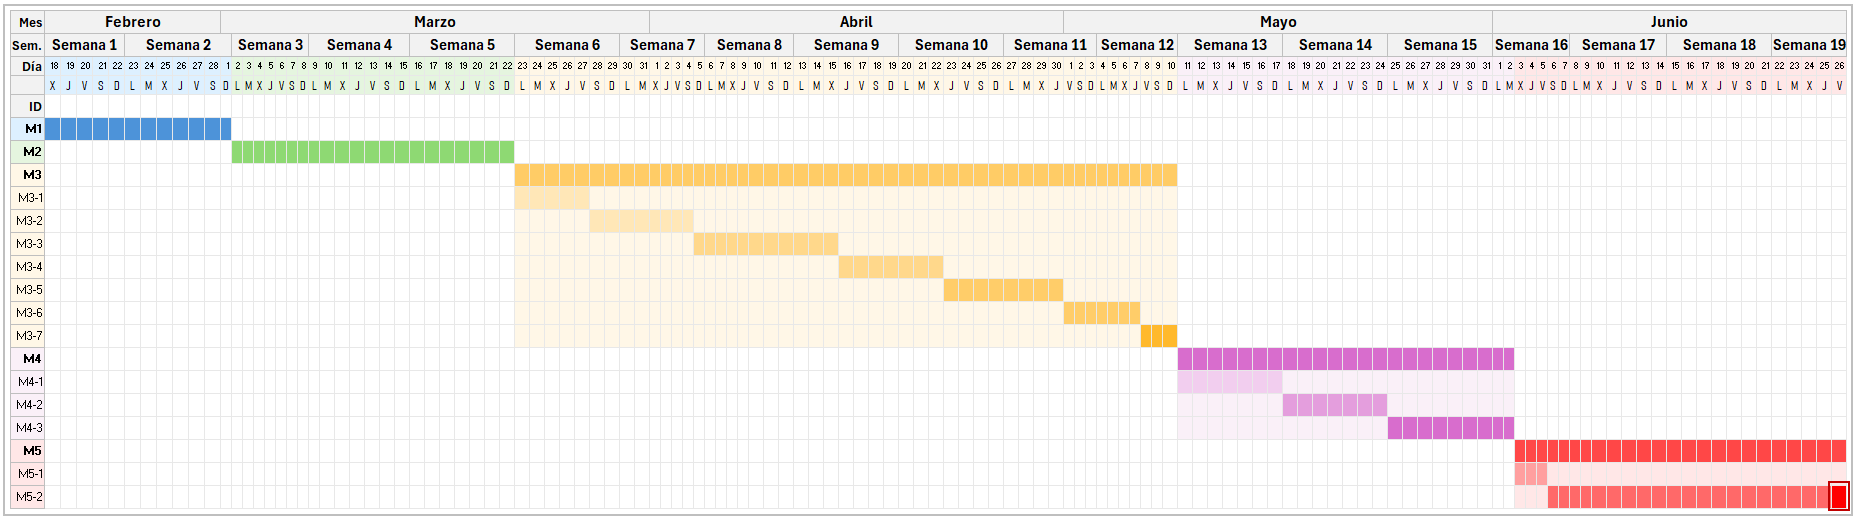
\includegraphics[width=1.1\textwidth]{images/planing.png}
\caption{Calendario de la planificación del proyecto (formato Gantt).}
\label{fig:planing}
\end{figure}


La planificación permite solapamientos controlados entre fases,
iniciando tareas como interpretabilidad o reconciliación jerárquica una
vez establecida una primera versión del modelo base. Esto optimiza el
tiempo disponible y reduce riesgos de acumulación de tareas en fases finales.

\newpage
\subsection{Gestión de riesgos del proyecto}

Se identifican los siguientes riesgos potenciales:

\begin{itemize}
\item
  \textbf{Coste computacional elevado del modelo LSTM}\\
  Probabilidad: Media\\
  Impacto: Alto\\
  Mitigación: uso de subconjuntos jerárquicos y reducción de
  dimensionalidad inicial.
\item
  \textbf{Dificultad en implementación de MinT}\\
  Probabilidad: Media\\
  Impacto: Medio\\
  Mitigación: priorizar Bottom-Up como método base garantizado.
\item
  \textbf{Rendimiento similar entre modelos sin diferencias
  significativas}\\
  Probabilidad: Media\\
  Impacto: Bajo\\
  Mitigación: enfocar el análisis en interpretabilidad y eficiencia
  computacional.
\item
  \textbf{Desviaciones en la planificación por complejidad técnica}\\
  Probabilidad: Media\\
  Impacto: Medio\\
  Mitigación: desarrollar primero un pipeline mínimo reproducible antes
  de optimizaciones avanzadas.
\item
  \textbf{Riesgo de data leakage en validación temporal\\
  }Probabilidad: Media\\
  Impacto: Alto\\
  Mitigación: validación walk-forward estricta y separación clara por
  horizonte.
\end{itemize}

La gestión de riesgos se integrará de forma dinámica en la planificación
temporal del proyecto. Cada hito técnico definido en la tabla de
planificación funcionará como punto de control para evaluar desviaciones
y activar medidas de mitigación, especialmente en las fases de modelado
y reconciliación jerárquica.

Cada riesgo será evaluado al final de su fase correspondiente, usando
los hitos técnicos como punto de control.

\newpage
\section{Impacto en sostenibilidad, ético-social y diversidad}

Desde la dimensión de sostenibilidad, una mejora en la precisión de los
modelos de predicción de demanda puede contribuir a reducir la
sobreproducción, el desperdicio de productos y los costes logísticos
asociados al transporte y almacenamiento, alineándose con objetivos de
eficiencia operativa y reducción del impacto ambiental.

Asimismo, se considerará la eficiencia computacional y energética de los
modelos desarrollados, analizando el impacto relativo de arquitecturas
más complejas como LSTM frente a modelos basados en árboles, en línea
con enfoques de inteligencia artificial sostenible.

En cuanto al comportamiento ético y responsabilidad social, el dataset
M5 se encuentra completamente anonimizado, sin incluir datos personales,
garantizando el respeto a la privacidad y el cumplimiento de normativas
de protección de datos. Además, se enfatiza que los modelos
desarrollados deben utilizarse como herramientas de apoyo a la toma de
decisiones y no como mecanismos automatizados excluyentes.

Finalmente, el uso de datasets públicos procedentes de plataformas
abiertas como Kaggle fomenta la accesibilidad, la igualdad de
oportunidades en investigación y la colaboración global, promoviendo la
diversidad en el desarrollo y evaluación de soluciones de inteligencia
artificial.

\newpage

\section*{Bibliografía}
\addcontentsline{toc}{section}{Bibliografía}

Chen, T., \& Guestrin, C. (2016). \emph{XGBoost: A scalable tree
boosting system}. Proceedings of the 22nd ACM SIGKDD International
Conference on Knowledge Discovery and Data Mining, 785--794.
https://doi.org/10.1145/2939672.2939785

Hyndman, R. J., Ahmed, R. A., Athanasopoulos, G., \& Shang, H. L.
(2011).\\
Optimal combination forecasts for hierarchical time series.\\
Computational Statistics \& Data Analysis, 55(9), 2579--2589.\\
https://doi.org/10.1016/j.csda.2011.03.006

Ke, G., Meng, Q., Finley, T., Wang, T., Chen, W., Ma, W., Ye, Q., \&
Liu, T.-Y. (2017). \emph{LightGBM: A highly efficient gradient boosting
decision tree}. Advances in Neural Information Processing Systems, 30.

Lundberg, S. M., \& Lee, S.-I. (2017). \emph{A unified approach to
interpreting model predictions}. Advances in Neural Information
Processing Systems, 30.

Makridakis, S., Spiliotis, E., \& Assimakopoulos, V. (2020). \emph{The
M5 accuracy competition: Results, findings and conclusions}.
International Journal of Forecasting, 36(1), 54--74.
https://doi.org/10.1016/j.ijforecast.2019.12.005

Walmart \& Kaggle. (2020). \emph{M5 Forecasting - Accuracy}
{[}Dataset{]}. Kaggle.
\url{https://www.kaggle.com/competitions/m5-forecasting-accuracy}

Wickramasuriya, S. L., Athanasopoulos, G., \& Hyndman, R. J. (2019).\\
Optimal forecast reconciliation for hierarchical and grouped time series
through trace minimization. International Journal of Forecasting, 35(2),
558--575. https://doi.org/10.1016/j.ijforecast.2018.11.006


\end{document}
